% File: main.tex
% Author: Auto-Intern GmbH
% Manuals template
\newcommand{\fach}{Digitaltechnikpraktikum }
\newcommand{\titelname}{Versuchsprotokoll }
\newcommand{\matrikel}{2016507006 }
\newcommand{\name}{Olbrich, Marie }

\newcommand{\matrikelpartner}{2016506999 }
\newcommand{\namepartner}{Hoffmann, Manuel }

\newcommand{\versuchsbezeichnung}{DT2 }
\newcommand{\versuchsname}{Schaltungstechnische Realisierung eines seriellen 4-Bit-Rechenwerkes }
\newcommand{\semester}{SS17 }
\newcommand{\datum}{02.05.2017 und 09.05.2017 }
\newcommand{\betreuer}{M.Sc. Kruse }
\newcommand{\dozent}{M.Sc. Richthofer }

\documentclass[a4paper, 11pt, fleqn, DIV=10, twoside, BCOR=10mm]{scrreprt}
\usepackage{diagbox}

%%%% Eingebundene Pakete %%%% 
\usepackage{xltxtra}

\usepackage{scrhack} 
\usepackage{xcolor}
\usepackage{color}
\usepackage{xfrac} % \sfrac{}{} für Brueche
\usepackage{graphicx}
\usepackage{float}
\usepackage{subcaption}
\usepackage{setspace}
\usepackage{wrapfig}
\usepackage{longtable}
\usepackage{geometry}
\usepackage{scrlayer-scrpage}
\usepackage{wallpaper}
\usepackage{ulem}
\usepackage{siunitx}
\usepackage{amsmath}
\usepackage{chngcntr}

%% Sorgt dafür, dass Kapitel neue Kapitel nicht auf einer neuen rechten Seite anfangen
\RedeclareSectionCommand[style=section,indent=0pt]{chapter}

%% Definition der Auto Intern Farben (Das AIschwarz wir im Fließtext nicht benutzt, stattdessen ist normales schwarz gesetzt (schwarze Tinte beim Druck günstiger)
\definecolor{THrot}{RGB}{228,0,30}
\definecolor{THblau}{RGB}{0,61,125}



%% Auto-Intern vereinfachte Befehle für Schriftarten
\newcommand{\mainfont}{\setmainfont{Lato-Regular.ttf}}
\newcommand{\LatoReg}{\setmainfont{Lato-Regular.ttf}}
\newcommand{\DaysOne}{\setmainfont{DaysOne-Regular.ttf}}
\newcommand{\LatoBold}{\setmainfont{Lato-Bold.ttf}}
\newcommand{\Avenir}{\setmainfont{AvenirLTStd-Book.otf}}
\newcommand{\LatoBlack}{\setmainfont{Lato-Black.ttf}}

%% Auto-Intern vereinfachte Befhele für Sprachwechsel eng - de
\newcommand{\Deutsch}{\usepackage[ngerman]{babel}
\renewcaptionname{ngerman}{\contentsname}{Inhaltsverzeichnis} % Standard: Inhaltsverzeichnis
\renewcaptionname{ngerman}{\listfigurename}{Abbildungsverzeichnis} % Standard: Abbildungsverzeichnis
\renewcaptionname{ngerman}{\listtablename}{Tabellenverzeichnis} % Standard: Tabellenverzeichnis
\renewcaptionname{ngerman}{\figurename}{Abbildung} % Standard: Abbildung
\renewcaptionname{ngerman}{\tablename}{Tabelle} % Standard: Tabelle
}


%% Auto-Intern vereinfachte Befehle für Textsatz
\newcommand{\Kursiv}[1]{\setmainfont{Lato-Italic.ttf}#1 \mainfont}
\newcommand{\Fett}[1]{\setmainfont{Lato-Bold.ttf}#1 \mainfont}
\newcommand{\FettKursiv}[1]{\setmainfont{Lato-BoldItalic.ttf}#1 \mainfont}
\newcommand{\Hoch}[1]{$^{\text{#1}}$}
\newcommand{\Tief}[1]{$_{\text{#1}}$}

%% Auto-Intern vereinfacht Befehle für Kapitel usw, um differenzierung zwischen Inhaltsverzeichnis und Text zu haben
\newcommand{\AItitlefont}{\LatoBold}
\newcommand{\Chapter}[1]{\chapter[#1]{\AItitlefont #1}}
\newcommand{\Section}[1]{\section[#1]{\AItitlefont #1}}
\newcommand{\Subsection}[1]{\subsection[#1]{\AItitlefont #1}}
\newcommand{\Subsubsection}[1]{\subsubsection[#1]{\AItitlefont #1}}
\newcommand{\Paragraph}[1]{\paragraph[#1]{\AItitlefont #1}}
\newcommand{\Subparagraph}[1]{\subparagraph[#1]{\AItitlefont #1}}

%% Einstellungen für Kopf- und Fußzeilen
\newcommand{\HeadAVier}{
\setlength{\footheight}{-1cm}
\setlength{\skip\footins}{5mm}
\setkomafont{pageheadfoot}{\setmainfont{Lato-Regular.ttf}} %Schriftart für Kopfzeile
\setkomafont{pagehead}{\setmainfont{Lato-Regular.ttf}} % Schriftart für Fußzeile
\pagestyle{scrheadings} % Seitenstil
\ihead{
\includegraphics[height=2cm]{../TemplateGraphics/Logo300.jpg}} % Innere Kopfzeile 7cm
\ohead{}
\chead{}
}


\newcommand{\ImpFootAVier}{
\ofoot{\LatoBlack \fach} % Äußere Fußzeile
\cfoot{}
\ifoot{
}}


\newcommand{\NormFoot}{
	\ifoot{\scriptsize% Innere Fußzeile
	\begin{tabular}{ll}
	\matrikel - \name\\%
	\matrikelpartner - \namepartner\\%
	Betreut durch: \betreuer
	\end{tabular}
	}
	\ofoot{\LatoBlack \fach\\ \versuchsbezeichnung \semester}
	\cfoot{\pagemark}
}

\newcommand{\EmptyFoot}{
\ifoot{}
\ofoot{}
\cfoot{}
}
%% Anderung der Schriftarten für Titelbeschriftungen
\usepackage{tocloft}
\setkomafont{disposition}{\AItitlefont\color{THblau}}  % farbe: ueberschrift
\renewcommand{\cfttoctitlefont}{\LatoBold \Large \color{THblau}}
\renewcommand{\cftpartfont}{\LatoReg}
\renewcommand{\cftchapfont}{\LatoReg}
\renewcommand{\cftsecfont}{\LatoReg}
\renewcommand{\cftsubsecfont}{\LatoReg}
\renewcommand{\cftsubsubsecfont}{\LatoReg}
\renewcommand{\cftparafont}{\LatoReg}
\renewcommand{\cftsubparafont}{\LatoReg}
\renewcommand{\cftfigfont}{\LatoReg}
%\renewcommand{\cftsubfigfont}{\LatoReg}
\renewcommand{\cfttabfont}{\LatoReg}
%\renewcommand{\cftsubtabfont}{\LatoReg}



\addtocontents{toc}{\protect\thispagestyle{scrheadings}}
\newcommand{\AVier}{
\HeadAVier
\ImpFootAVier
\AItitlefont
\addtolength{\wpYoffset}{-3cm}
\ThisCenterWallPaper{0.7}{../TemplateGraphics/Kopf.pdf}%
{\color{white}.}\\
\vspace{3.5cm}
\begin{center}
{{\huge \titelname  zu \versuchsbezeichnung} \\ \LatoReg \versuchsname\\ \vspace{40mm} durchgeführt von \\ \Fett \matrikel \LatoReg \name \\ \Fett \matrikelpartner \LatoReg \namepartner \\ im \semester am \datum \\ \vspace{10mm} Betreut durch: \betreuer \\ Dozent: \dozent}
\end{center}
\newpage
\mainfont
\NormFoot
\tableofcontents
\newpage
\setcounter{page}{1}
\ohead{\thepage}
}

\Deutsch
\begin{document} 
\AVier
\begin{center}
\chapter{Vorbereitende Aufgaben}
\section{Addierer}
\subsection{Halbaddierer}
\begin{tabular}{c|c||c|c}
S1&S2&E&Ü\\
\hline
0&0&0&0\\
0&1&1&0\\
1&0&1&0\\
1&1&0&1\\
\end{tabular}
\captionof{table}{Wahrheitstabelle Halbaddierer}
\vspace{15mm}
\begin{tabular}{c|c|c}
\diagbox{S2}{S1}&0&1\\
\hline
0&0&1\\
\hline
1&1&0\\
\end{tabular}
\captionof{table}{KV-Diagramm Halbaddierer Ergebnis}
\vspace{15mm}
\begin{tabular}{c|c|c}
\diagbox{S2}{S1}&0&1\\
\hline
0&0&0\\
\hline
1&0&1\\
\end{tabular}
\captionof{table}{KV-Diagramm Halbaddierer Übertrag}
\begin{equation}
	E:=(\overline{S1} \wedge S2) \vee (S1 \wedge \overline{S2})
\end{equation}
\begin{equation}
	"U:=S1 \wedge S2
\end{equation}
\newpage
\subsection{Volladdierer}
\begin{tabular}{c|c|c||c|c}
S1&S2&ÜE&E&ÜA\\
\hline
0&0&0&0&0\\
0&0&1&1&0\\
0&1&0&1&0\\
0&1&1&0&1\\
1&0&0&1&0\\
1&0&1&0&1\\
1&1&0&0&1\\
1&1&1&1&1\\
\end{tabular}
\captionof{table}{Wahrheitstabelle Volladdierer}
\vspace{15mm}
\begin{tabular}{c|c|c}
\diagbox{S1S2}{ÜE}&0&1\\
\hline
00&0&1\\
\hline
01&1&0\\
\hline
11&0&1\\
\hline
10&1&0\\
\end{tabular}
\captionof{table}{KV-Diagramm Volladdierer Ergebnis}
\vspace{15mm}
\begin{tabular}{c|c|c}
\diagbox{S1S2}{ÜE}&0&1\\
\hline
00&0&0\\
\hline
01&0&1\\
\hline
11&1&1\\
\hline
10&0&1\\
\end{tabular}
\captionof{table}{KV-Diagramm Volladdierer Übertrag Ausgang}
	\begin{equation}
	E:= ("UE \wedge \overline{S1} \wedge \overline{S2}) \vee (\overline{"UE} \wedge \overline{S1} \wedge S2) \vee ("UE \wedge S1 \wedge S2) \vee ("UE \wedge S1 \wedge \overline{S2})
	\end{equation}
	\begin{equation}
	"UA:= (S1 \wedge S2) \vee ("UE \wedge S2) \vee ("UE \wedge S1)
	\end{equation}
\section{Subtrahierer}
\subsection{Halbsubtrahierer}
\begin{tabular}{c|c||c|c}
S1&S2&E&Ü\\
\hline
0&0&0&0\\
0&1&1&1\\
1&0&1&0\\
1&1&0&0\\
\end{tabular}
\captionof{table}{Wahrheitstabelle Halbsubtrahierer}
\vspace{15mm}
\begin{tabular}{c|c|c}
\diagbox{M}{S}&0&1\\
\hline
0&0&1\\
\hline
1&1&0\\
\end{tabular}
\captionof{table}{KV-Diagramm Halbsubtrahierer Differenz}
\vspace{15mm}
\begin{tabular}{c|c|c}
\diagbox{M}{S}&0&1\\
\hline
0&0&1\\
\hline
1&0&0\\
\end{tabular}
\captionof{table}{KV-Diagramm Halbsubtrahierer Entleihung}
\begin{equation}
	D:= (S \wedge \overline{M}) \vee (\overline{S} \wedge M)
\end{equation}
\begin{equation}
	E:= S \wedge \overline{M}
\end{equation}
\newpage
\subsection{Vollsubtrahierer}
\begin{tabular}{c|c|c||c|c}
M&S&EE&D&EA\\
\hline
0&0&0&0&0\\
0&0&1&1&1\\
0&1&0&1&1\\
0&1&1&0&1\\
1&0&0&1&0\\
1&0&1&0&0\\
1&1&0&0&0\\
1&1&1&1&1\\
\end{tabular}
\captionof{table}{Wahrheitstabelle Vollsubtrahierer}
\vspace{15mm}
\begin{tabular}{c|c|c}
\diagbox{MS}{EE}&0&1\\
\hline
00&0&1\\
\hline
01&1&0\\
\hline
11&0&1\\
\hline
10&1&0\\
\end{tabular}
\captionof{table}{KV-Diagramm Halbaddierer Differenz}
\vspace{15mm}
\begin{tabular}{c|c|c}
\diagbox{MS}{EE}&0&1\\
\hline
00&0&1\\
\hline
01&1&1\\
\hline
11&0&1\\
\hline
10&0&0\\
\end{tabular}
\captionof{table}{KV-Diagramm Vollsubtrahierer Entleihung Ausgang}
	\begin{equation}
	D:= (EE \wedge \overline{M} \wedge \overline{S}) \vee (\overline{EE} \wedge \overline{M} \wedge S) \vee (EE \wedge M \wedge S) \vee (\overline{EE} \wedge M \wedge \overline{S})
	\end{equation}
	\begin{equation}
	EA:= (EE \wedge \overline{M}) \vee (\overline{M} \wedge S) \vee (EE \wedge S)
	\end{equation}
\end{center}
\newpage
\section{Halb- und Volladdierer}
Der Halbaddierer hat zwei, der Volladdierer drei Eingänge. Daher kann der Halbaddierer nur zwei einstellige Dualzahlen addieren, ohne einen Übertrag zu berücksichtigen. Da der Volladdierer einen Eingang mehr hat, kann er drei einstellige Dualzahlen, bzw. zwei mehrstellige Zahlen addieren. Beide haben je einen Ausgang für das Ergebnis und einen für den Übertrag.
\section{Anzahl D-Flipflops}
Man braucht fünf D-Flipflops, weil man 4-Bit-Dualzahlen und einen Übertrag berücksichtigen muss.
\section{Taktzyklen Systemtakt}
Man benötigt fünf Taktzyklen, damit die vier Ergebnisse und der Übertrag durch das Schieberegister geschoben werden können.
\begin{center}
\newpage
\end{center}
\section{Blockschaltbild 1}
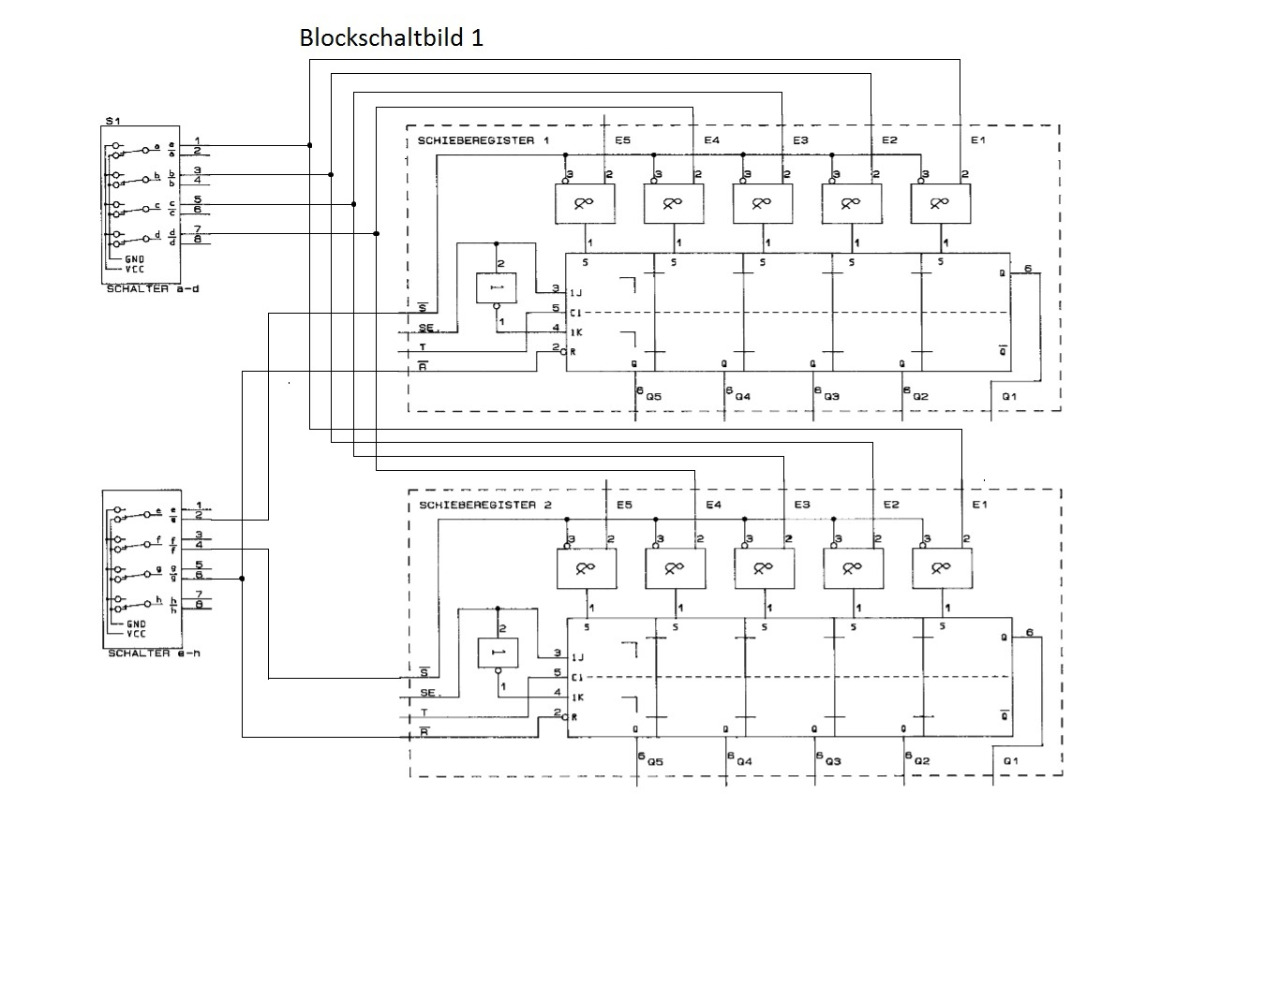
\includegraphics[width=1.35\columnwidth]{DT2Graphics/Blockschaltbild1.jpeg}
\section{Blockschaltbild 2}
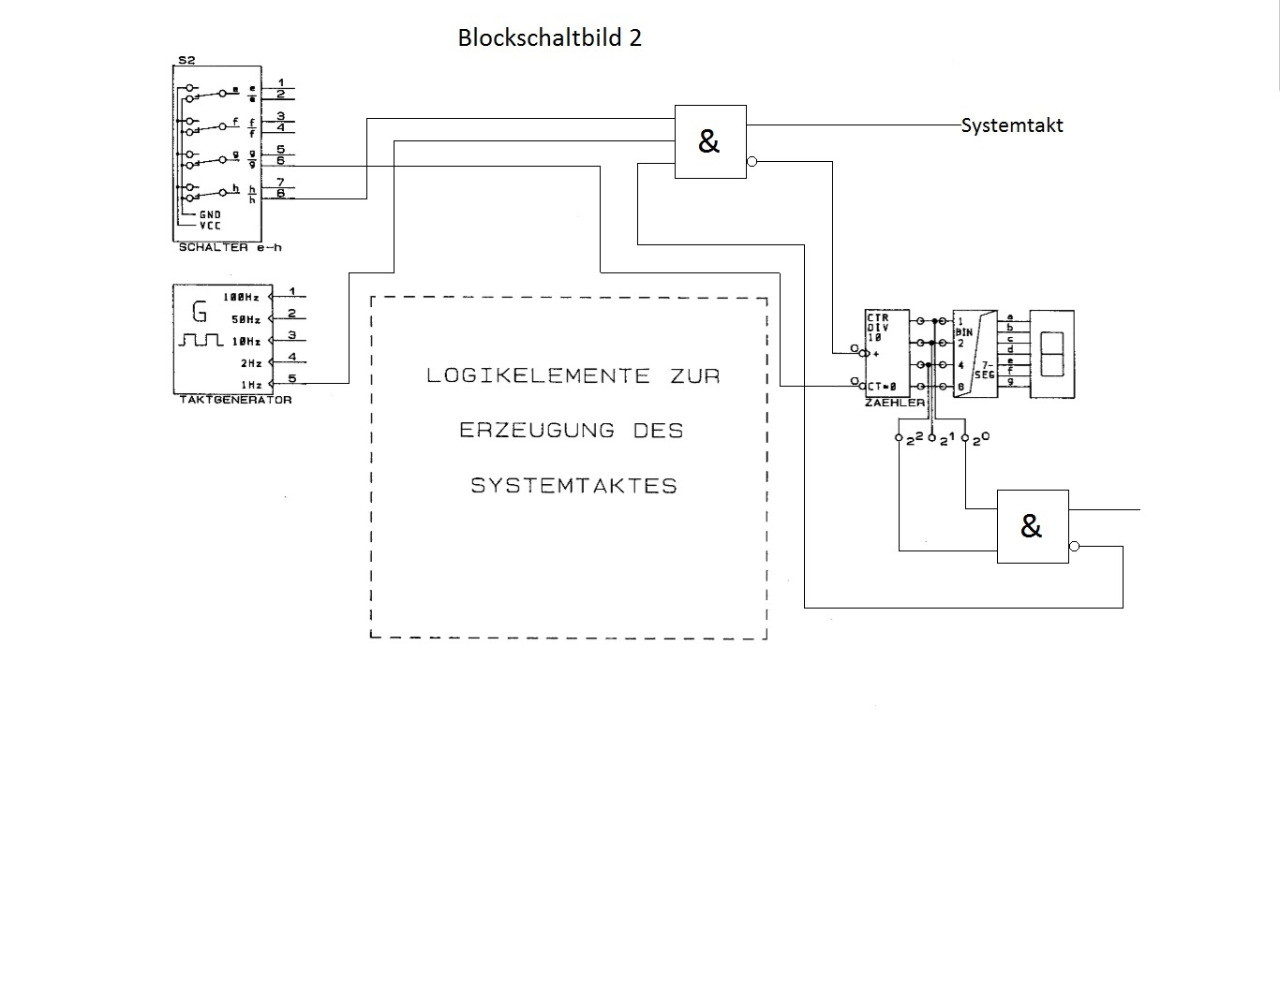
\includegraphics[width=1.25\columnwidth]{DT2Graphics/Blockschaltbild2.jpeg}
\section{Blockschaltbild 3}
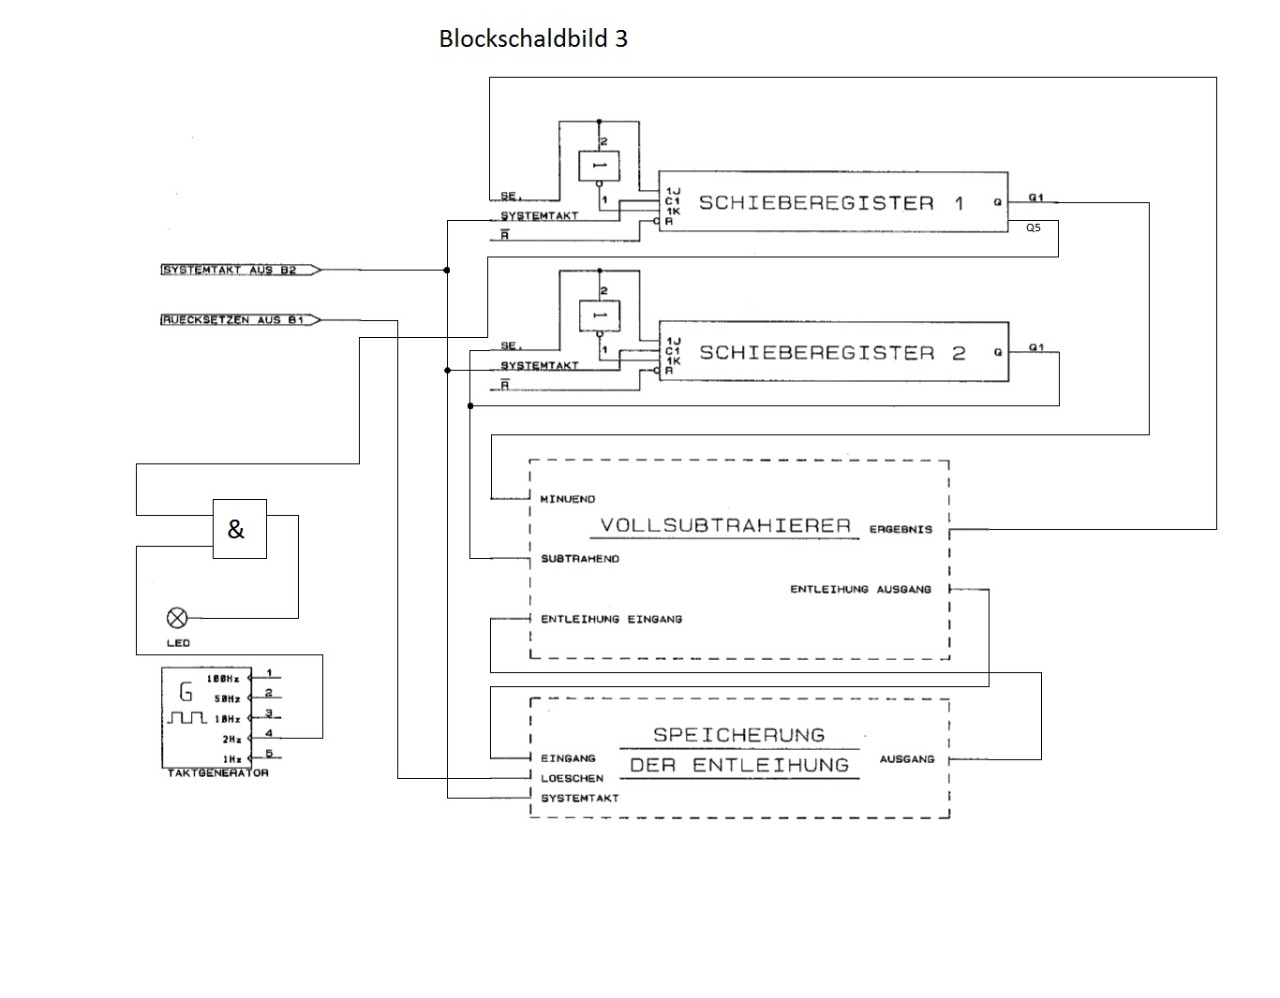
\includegraphics[width=1.2\columnwidth]{DT2Graphics/Blockschaltbild3.jpeg}
\newpage
\chapter{Kritische Schlussbetrachtung}
\section{Olbrich, Marie}
 In Versuch DT2 ging es um die schaltungstechnische Realisierung eines seriellen, 4-Bit-Rechenwerkes. Es sollen zunächst zwei 4-Bit-Dualzahlen in zwei Schieberegister parallel eingeschrieben werden, welche anschließend seriell mittels eines Vollsubtrahierers subtrahiert werden sollen. Das Ergebnis soll in einem der beiden Schieberegister gespeichert werden. Außerdem ist ein Systemtakt zu erzeugen, damit das Ergebnis nicht nocheinmal verrechnet wird.\par
Dazu sollten zunächst drei einzelne Schaltungen entwickelt werden. Die erste Schaltung dient zur Einlesung der beiden Dualzahlen in die Schieberegister. Mit Hilfe der zweiten Schaltung wird ein Systemtakt erzeugt. Die dritte Schaltung enthält die Elemente der vorherigen beiden und verbindet sie mit einem Vollsubtrahierer. Die Entleihung wird auch gespeichert und bei einem negativen Ergebnis soll eine LED leuchten. Ist das Ergebnis negativ, müsste noch das Zweierkomplement gebildet werden, weshalb das angezeigte Ergebnis nicht korrekt ist.\par
Am Versuchstag sollten die einzelnen Teilschaltungen auf einem Board (siehe Bild) aufgebaut und in ihrer Funktion vorgeführt werden. Es traten keine Probleme auf und der Subtrahierer funktionierte auf Anhieb einwandfrei.\par
Die vorbereitenden Aufgaben konnten ebenfalls ohne größere Probleme in der vorgegebenen Zeit gelöst werden.


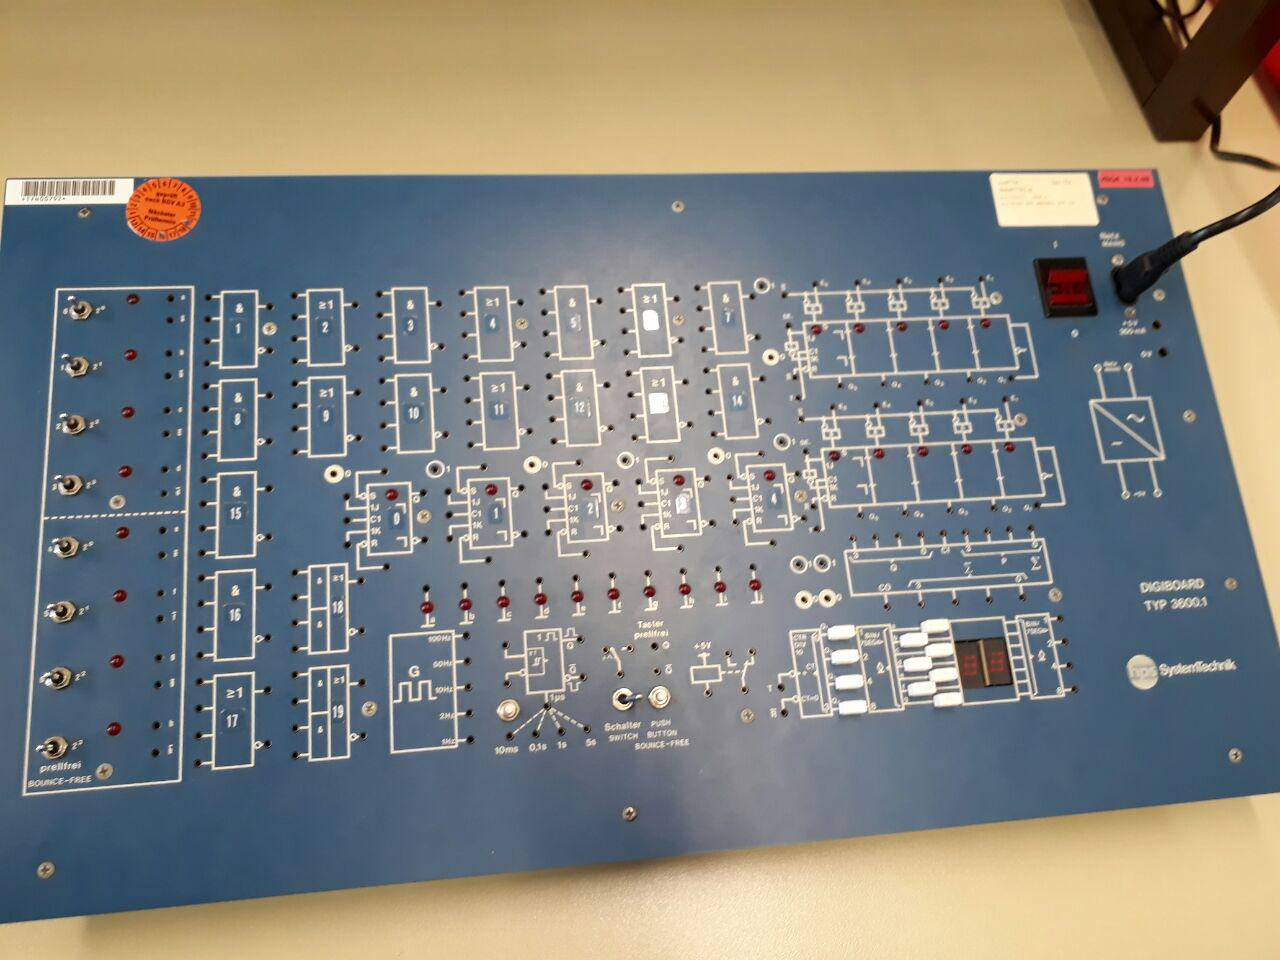
\includegraphics[width=0.75\columnwidth]{DT2Graphics/Board.jpg}

\section{Hoffmann, Manuel}
 

	Schaltungstechnische Realisierung eines seriellen, 4-Bit Rechenwerkes	
	
	Zu beginn des Versuchs DT2 wird, je nach Gruppe, festgelegt ob ein 4-Bit 
	Addierer oder Subtrahierer zu bearbeiten ist.
	Die unterschiedliche Aufgabenstellung, je nach Gruppe, kommt dabei erst
	in der Vorbereitenden Aufgabe 1.8 (Blockschaltbild 3) zu tragen.
	Im vorliegendem Fall wird der Subtrahierer erstellt.
	
	Die Vorbereitenden Aufgaben beginnen mit grundsätzlichem wie z.B. die 					Einarbeitung in Rechenschaltung, Flipflop-Arten(1.1) oder die Unterschiede 
	zwischen Halb- und Voll-Addierer bzw. Subtrahierer(1.3). 
	Im weiteren Verlauf muss man, nach den Regeln der Schaltungssynthese, 
	Voll- und Halb-Addierer sowie Subtrahierer entwerfen(1.2).
	Anschließend sind noch die Fragen nach der anzahl der benötigten
	D-Flipflops je Schieberegister(1.4) und der Anzahl von Tacktzyklen des 
	Systemtakts(1.5) zu beantworten.
	
	Weiterführend ist das erste Blockschaltbild zu vervollständigen.
	Hierbei wird die Verschaltung der Schieberegister zur Aufnahme der 
	Summanden, im Fall des Addierers, bzw. des Subtrahenden und Minuenden, 
	im Fall des Subtrahierers, und des Ergebnisses.
	Dabei ist speziell auf die Schalter Verkabelung zum freischalten und zum 
	löschen der Register zu achten.
	
	Im Blockschaltbild 2 wird eine Schaltung zur Generierung des Systemtaktes
	erstellt. Auch dabei ist auf den korrekten Anschluss der Schalter zu 
	achten um die vorgegebenen Funktionen zu gewährleisten. 
	
	Das dritte Blockschaltbild, Aufgabe 1.8b, zeigt die schaltung 
	des Vollsubtrahierers.
	Bedingt durch den Aufbau des Vollsubtrahierers sind einige Besonderheiten
	zu beachten. Zum einen muss die Speicherung der Entleihung gesondert im 
	Schaltbild verkabelt werden. Des weiteren soll laut Aufgabenstellung eine 
	LED eingebunden werden die im Falle eines negativen Rechenergebnisses 
	mit einer Frequenz von 2 Hz blinkt. Wie zuvor ist im allgemeinen auch wieder
	auf das anschließen der Schalter wie vorgegeben zu achten.
	
	Am Versuchstag sind die einzelnen Schaltungen gemäß der zuvor angefertigten 
	Blockschaltbilder aufzubauen und zu Prüfen.
	Dabei ist jede Teilschaltung sowie das gesamte Rechenwerk vorzuführen.
	Bei Korrekten Schaltzeichnungen sollte der praktische Aufbau der Schaltungen
	kein Problem darstellen. 
%%%%%%%%%%%%%%%%%%%%%%%%%%%%%%%%%%%%%%%%%%%%%%%%%%%%%%%%%%%%%%%%%%%%%%%%%%%%%%%%%%%%%%%
%%%%%%%%%%%%%%%%%%%%%%%%%%%%%%%%%%%%%%%%%%%%%%%%%%%%%%%%%%%%%%%%%%%%%%%%%%%%%%%%%%%%%%%
%%%%%%%%%%%%%%%%%%%%%%%%%%%%%%%%%%%%%%%%%%%%%%%%%%%%%%%%%%%%%%%%%%%%%%%%%%%%%%%%%%%%%%%
%%%%%%%%%%%%%%%%%%%%%%%%%%%%% Hier fängt der Text an %%%%%%%%%%%%%%%%%%%%%%%%%%%%%%%%%%
%%%%%%%%%%%%%%%%%%%%%%%%%%%%%%%%%%%%%%%%%%%%%%%%%%%%%%%%%%%%%%%%%%%%%%%%%%%%%%%%%%%%%%%
%%%%%%%%%%%%%%%%%%%%%%%%%%%%%%%%%%%%%%%%%%%%%%%%%%%%%%%%%%%%%%%%%%%%%%%%%%%%%%%%%%%%%%%
%%%%%%%%%%%%%%%%%%%%%%%%%%%%%%%%%%%%%%%%%%%%%%%%%%%%%%%%%%%%%%%%%%%%%%%%%%%%%%%%%%%%%%%
\end{document}